\section{一阶方程的解析求解}
\label{sec:ivp-first-order}

有了解的标准，就可以着手求解。多数方程写不出公式，能够求解的方程靠的是右端的特殊形式：或者时间与状态可以分开，或者换一个未知量后可以分开。下面两小节分别处理这两种情况。一阶线性方程的积分因子在第~\ref{chap:linear-differential-systems}章统一介绍。

\subsection{分离变量}
\label{sec:ivp-separable}

若右端是时间的函数与状态的函数的乘积，
\begin{equation}
 \dot{x}=a(t)\,b(x),
 \label{eq:ivp-separable}
\end{equation}
则称方程为\term{可分离方程}（separable equation）。这里$a:T\to\mathbb{R}$连续，$b:D\to\mathbb{R}$连续，$T$是区间，$D$是开区间。

\paragraph{从形式计算到定理}
教科书里常见的写法是把方程改写成$\mathrm{d}x/b(x)=a(t)\,\mathrm{d}t$，再两边积分。这个写法方便记忆，却藏着两个问题：除以$b(x)$要求$b(x)\neq 0$；积分之后得到的是一个等式，把$x$解出来还需要函数可逆。下面的定理把这两点写清楚。

\begin{theorem}[分离变量]
 \label{thm:ivp-separation}
 考虑式~\eqref{eq:ivp-separable}与初值$x(t_0)=x_0$，$t_0\in T$，$x_0\in D$。
 \begin{enumerate}
 \item 若$b(x_0)=0$，则常值函数$x\equiv x_0$是$T$上的解。
 \item 若$b(x_0)\neq 0$，记$D_0\subseteq D$为包含$x_0$且$b$在其上无零点的最大开区间，定义
 \begin{equation}
 B(x)=\int_{x_0}^{x}\frac{\mathrm{d}\xi}{b(\xi)},\quad x\in D_0,\qquad
 A(t)=\int_{t_0}^{t}a(s)\,\mathrm{d}s,\quad t\in T.
 \label{eq:ivp-separation-primitives}
 \end{equation}
 则$B$是$D_0$上严格单调的连续可微函数，其值域$J=B(D_0)$是包含$0$的开区间。对任何包含$t_0$的区间$I\subseteq T$，只要$A(I)\subseteq J$，函数
 \begin{equation}
 x(t)=B^{-1}\bigl(A(t)\bigr)
 \label{eq:ivp-separation-solution}
 \end{equation}
 就是$I$上的解；并且$I$上任何取值于$D_0$的解都等于式~\eqref{eq:ivp-separation-solution}。
 \end{enumerate}
\end{theorem}

\begin{proof}
 第一条可直接验证：常值函数导数为零，而右端$a(t)b(x_0)=0$。

 下面证第二条。在$D_0$上$b$连续且无零点，由介值定理$b$不变号，所以$1/b$连续且不变号。由微积分基本定理，$B$连续可微，$B'=1/b$，于是$B$严格单调。严格单调的连续函数把开区间映成开区间，又$B(x_0)=0$，所以$0\in J$。

 反函数$B^{-1}:J\to D_0$连续可微，导数为$1/B'$，即
 \[
 (B^{-1})'(y)=b\bigl(B^{-1}(y)\bigr).
 \]
 若$A(I)\subseteq J$，由链式法则，式~\eqref{eq:ivp-separation-solution}定义的$x$满足
 \[
 \dot{x}(t)=b\bigl(B^{-1}(A(t))\bigr)\,\dot{A}(t)=b\bigl(x(t)\bigr)\,a(t).
 \]
 又$x(t_0)=B^{-1}(0)=x_0$，所以$x$是解。

 反过来，设$x:I\to D_0$是任意解。由链式法则，
 \[
 \frac{\mathrm{d}}{\mathrm{d}t}B\bigl(x(t)\bigr)=\frac{\dot{x}(t)}{b(x(t))}=a(t).
 \]
 右端连续，从$t_0$积分，得到$B(x(t))-B(x_0)=A(t)$，即$B(x(t))=A(t)$。这说明$A(I)\subseteq J$，并且$x(t)=B^{-1}(A(t))$。
\end{proof}

定理的条件各有用处。$a$、$b$连续保证$A$、$B$有定义。$D_0$的选取把$x_0$所在的一段状态与$b$的零点隔开，保证能除。条件$A(I)\subseteq J$决定存在区间：式~\eqref{eq:ivp-separation-solution}只在$A(t)$落在$J$中时有意义。最后一句中的“取值于$D_0$”是一个实际的限制，解是否会离开$D_0$，要看$b$在$D_0$端点附近的行为，本小节末尾再讨论。

\paragraph{Logistic方程的完整求解}
对式~\eqref{eq:ivp-logistic}，$a\equiv 1$，$b(x)=x(1-x)$，$t_0=0$。$b$的零点是$0$和$1$，它们给出两个平衡解，并把实轴分成三段：$(-\infty,0)$、$(0,1)$、$(1,\infty)$。$x_0$落在哪一段，$D_0$就是哪一段。

先把被积函数拆成部分分式：
\[
 \frac{1}{\xi(1-\xi)}=\frac{1}{\xi}+\frac{1}{1-\xi}.
\]
在每一段上$\xi/(1-\xi)$保持固定符号，逐项积分得到
\[
 B(x)=\Bigl[\ln\Bigl\lvert\frac{\xi}{1-\xi}\Bigr\rvert\Bigr]_{x_0}^{x}
 =\ln\frac{x(1-x_0)}{x_0(1-x)}.
\]
这里$A(t)=t$，令$B(x)=t$并解出$x$：
\begin{equation}
 x(t)=\frac{x_0\mathrm{e}^{t}}{1-x_0+x_0\mathrm{e}^{t}}.
 \label{eq:ivp-logistic-general-solution}
\end{equation}
代入$x_0=0.1$，分子分母同乘$10$，就得到式~\eqref{eq:ivp-logistic-solution}。

公式相同，存在区间却随初值而不同。定理告诉我们，存在区间由$J$决定，所以只要算出$B$的值域。取$x_0=2$，$D_0=(1,\infty)$，这时
\[
 B(x)=\ln\frac{x}{2(x-1)}.
\]
当$x\to 1^{+}$时$B\to+\infty$，当$x\to+\infty$时$B\to-\ln 2$，所以$J=(-\ln 2,\infty)$，存在区间是$I=(-\ln 2,\infty)$。类似地，取$x_0=-0.5$，$D_0=(-\infty,0)$，
\[
 B(x)=\ln\frac{3x}{x-1}.
\]
当$x\to 0^{-}$时$B\to-\infty$，当$x\to-\infty$时$B\to\ln 3$，所以$J=(-\infty,\ln 3)$，$I=(-\infty,\ln 3)$。

\begin{BookInlineTable}
 \centering
 \caption{Logistic方程$\dot{x}=x(1-x)$的三种初值}
 \label{tab:ivp-logistic-regimes}
 \begin{tabular}{llll}
 \toprule
 初值$x_0$ & $D_0$ & $J=B(D_0)$ & 存在区间$I$ \\
 \midrule
 $0.1$ & $(0,1)$ & $\mathbb{R}$ & $\mathbb{R}$ \\
 $2$ & $(1,\infty)$ & $(-\ln 2,\infty)$ & $(-\ln 2,\infty)$ \\
 $-0.5$ & $(-\infty,0)$ & $(-\infty,\ln 3)$ & $(-\infty,\ln 3)$ \\
 \bottomrule
 \end{tabular}
\end{BookInlineTable}

图~\ref{fig:ivp-logistic-regimes}画出了这三条解。在$x_0=2$的解上，往回追溯，在$t=-\ln 2$之前状态是无穷大；在$x_0=-0.5$的解上，$t$增加到$\ln 3$时状态趋于$-\infty$。右侧的竖线称为相线，它把自治标量方程的信息压缩到状态轴上：两个点是平衡解，箭头表示状态运动的方向，方向由$b(x)$的符号决定。

\begin{BookInlineFigure}
 \centering
 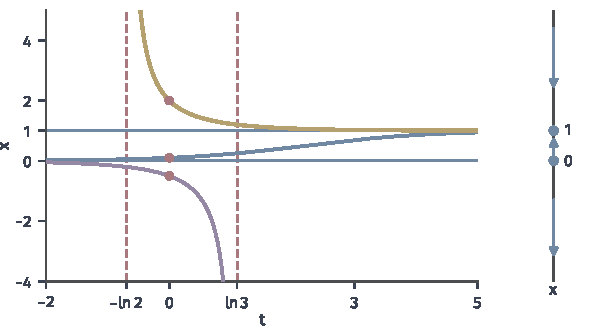
\includegraphics[width=104mm]{figures/06-differential-equations/01-ordinary-differential-equations/matplotlib/ivp-logistic-regimes/figure.pdf}
 \caption{$\dot{x}=x(1-x)$的三类解。蓝线$x_0=0.1$的解在全实轴上存在，黄线$x_0=2$的解在$t\downarrow-\ln 2$时趋于$+\infty$，紫线$x_0=-0.5$的解在$t\uparrow\ln 3$时趋于$-\infty$。水平蓝线是平衡解$x\equiv 0$与$x\equiv 1$，红色虚线是两个爆炸时刻。右侧相线上的箭头是$\dot{x}$的符号。}
 \label{fig:ivp-logistic-regimes}
\end{BookInlineFigure}

\paragraph{$a(t)$是一个改了刻度的时钟}
时间因子$a(t)$的作用可以这样看。令$\chi(s)$是自治方程$\chi'=b(\chi)$的解，$\chi(0)=x_0$，这个解由定理（取$a\equiv 1$）给出，满足$B(\chi(s))=s$。比较式~\eqref{eq:ivp-separation-solution}，有$x(t)=\chi(A(t))$。也就是说，时间因子只是把自治解放到一个新的时钟$s=A(t)$上走，时钟的快慢由$a(t)$决定，$a(t)<0$时时钟倒着走。

例如$\dot{x}=2tx^2$，$x(0)=1$。这里$a(t)=2t$，$b(x)=x^2$，$D_0=(0,\infty)$，计算得
\[
 A(t)=t^2,\qquad B(x)=1-\frac{1}{x},\qquad J=(-\infty,1).
\]
由$B(x)=A(t)$解出$x=1/(1-t^2)$，条件$A(t)\in J$即$t^2<1$，存在区间是$(-1,1)$。这正是第~\ref{sec:ivp-verification}节的爆炸解$1/(1-s)$放到时钟$s=t^2$上。代回检验：$\dot{x}=2t/(1-t^2)^2=2tx^2$，$x(0)=1$。

\paragraph{隐式解什么时候解得出}
积分后得到的是$B(x)=A(t)$，它未必能写成初等函数。考虑
\[
 \dot{x}=\frac{2t}{1+\mathrm{e}^{x}},\qquad x(0)=0.
\]
这里$a(t)=2t$，$b(x)=1/(1+\mathrm{e}^{x})$无零点，$D_0=\mathbb{R}$。计算两个原函数：
\[
 B(x)=\int_0^{x}(1+\mathrm{e}^{\xi})\,\mathrm{d}\xi=x+\mathrm{e}^{x}-1,\qquad A(t)=t^2.
\]
于是解由$x+\mathrm{e}^{x}-1=t^2$确定，这个方程没有初等的解出形式。但$B$严格递增，值域是整个$\mathbb{R}$，定理保证对每个$t$都恰有一个$x$，解在全实轴上存在。$t=1$时要解$x+\mathrm{e}^{x}=2$，数值求根得$x\approx 0.443$，这是图~\ref{fig:ivp-implicit-solve}中的紫点。

\begin{BookInlineFigure}
 \centering
 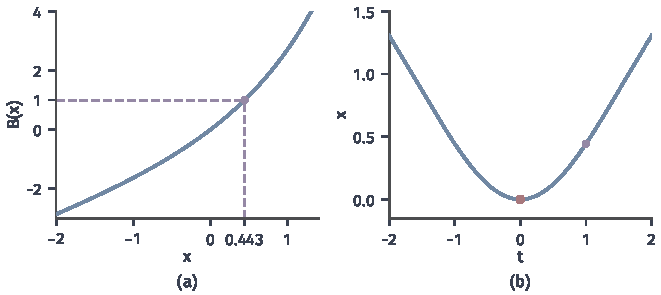
\includegraphics[width=112mm]{figures/06-differential-equations/01-ordinary-differential-equations/matplotlib/ivp-implicit-solve/figure.pdf}
 \caption{隐式解$x+\mathrm{e}^{x}-1=t^2$。(a)函数$B(x)=x+\mathrm{e}^{x}-1$严格递增，水平线$B=1$（$t=\pm 1$时的$A(t)$）与曲线恰交于一点，$x\approx 0.443$。(b)由此逐点解出的解曲线，红点是初值$x(0)=0$，紫点对应$t=1$。}
 \label{fig:ivp-implicit-solve}
\end{BookInlineFigure}

更一般地，积分可能给出一个形如$G(t,x)=C$的关系。在一点附近能把$x$解成$t$的函数，靠的是隐函数定理的条件$\partial_x G\neq 0$，可参考\BookChapterRef{chap:implicit-inverse-functions}{卷二第22章“隐函数与反函数”}。对分离变量，$G(t,x)=B(x)-A(t)$，所以$\partial_xG=1/b(x)\neq 0$，这就是定理中$B$可逆的原因。圆$x^2+t^2=1$对应的$G=x^2+t^2$在$t=\pm 1$处$\partial_xG=2x=0$，解在那里走不下去，与图~\ref{fig:ivp-implicit-branches}一致。

\paragraph{零点上可能发生什么}
定理第一条只说零点给出一个解，并没有说这是唯一的解。考虑
\[
 \dot{x}=2\sqrt{\lvert x\rvert},\qquad x(0)=0.
\]
$x\equiv 0$当然是解。若只在$x>0$上按定理计算，$B'(x)=1/(2\sqrt{x})$，得到$\sqrt{x}=t-c$，即$x=(t-c)^2$，$t\geq c$。这条曲线在$t=c$处斜率为零，可以和零解光滑地接起来：对任何$c\geq 0$，
\begin{equation}
 x_c(t)=\begin{cases}0,&t<c,\\(t-c)^2,&t\geq c\end{cases}
 \label{eq:ivp-sqrt-family}
\end{equation}
都连续可微，并满足方程：$t\geq c$时$\dot{x}_c=2(t-c)=2\sqrt{x_c}$。

\begin{BookInlineFigure}
 \centering
 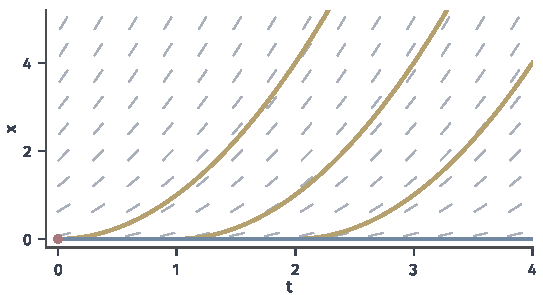
\includegraphics[width=92mm]{figures/06-differential-equations/01-ordinary-differential-equations/matplotlib/ivp-lost-solutions/figure.pdf}
 \caption{$\dot{x}=2\sqrt{\lvert x\rvert}$，$x(0)=0$的多个解。蓝线是平衡解$x\equiv 0$，黄线是式~\eqref{eq:ivp-sqrt-family}中$c=0,\,1,\,2$的解，它们在零解上停留一段时间后离开。}
 \label{fig:ivp-lost-solutions}
\end{BookInlineFigure}

图~\ref{fig:ivp-lost-solutions}显示，从同一个初值出发有无穷多条解。若先除以$\sqrt{x}$，就只会得到$x=t^2$这一条，把$x\equiv 0$和其余的解都丢掉了。所以分离变量的第一步是列出$b$的全部零点，分别处理；这个例子还说明，处理完零点也不代表解已经找全。什么条件能保证解唯一，是第~\ref{chap:ode-existence-continuation}章的主题。

\paragraph{时间等于路程除以速度}
解能否走到$b$的零点，能否走到无穷远，都可以从定理的公式读出来。取$a\equiv 1$，$B(x)=t-t_0$可以写成
\begin{equation}
 t-t_0=\int_{x_0}^{x(t)}\frac{\mathrm{d}\xi}{b(\xi)}.
 \label{eq:ivp-travel-time}
\end{equation}
这和“时间等于路程除以速度”是同一回事：$b(\xi)$是状态走到$\xi$处的速度，$1/b$是走单位路程的耗时，经过的时间就是$1/b$曲线下的面积。图~\ref{fig:ivp-slowness}展示了三种情形。

\begin{BookInlineFigure}
 \centering
 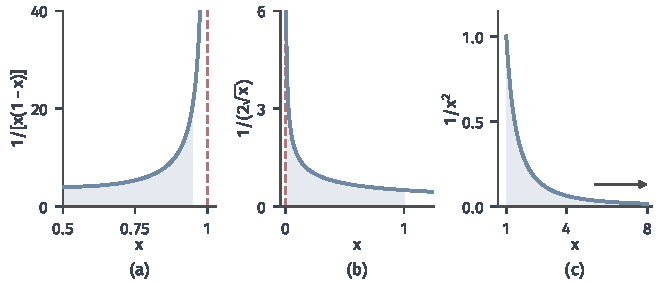
\includegraphics[width=112mm]{figures/06-differential-equations/01-ordinary-differential-equations/matplotlib/ivp-slowness/figure.pdf}
 \caption{经过时间等于$1/b$曲线下的面积。(a)$b=x(1-x)$：$1/b$在$x=1$处的积分发散，浅蓝区是从$0.5$到$0.95$所用的时间，走到$1$需要无穷长时间。(b)$b=2\sqrt{x}$：在$x=0$处的奇异可积，从$0$走到$1$只用时间$1$。(c)$b=x^2$：$1/x^2$在无穷远可积，从$1$走到无穷远只用时间$1$。}
 \label{fig:ivp-slowness}
\end{BookInlineFigure}

(a)中$b$在零点附近像线性函数，$1/b$像$1/\lvert x-1\rvert$，积分对数发散，解需要无穷长的时间才能接近平衡，这和$x_0=0.1$的解只是逐渐趋于$1$一致。(b)中$b$在零点附近比线性函数大得多，$1/b$可积，走到零点只需有限时间，于是解可以到达零点甚至从零点离开，这就是图~\ref{fig:ivp-lost-solutions}的现象。(c)中速度增长得足够快，$1/b$在无穷远可积，到达无穷远只需有限时间，这是爆炸的原因。

\subsection{变量代换}
\label{sec:ivp-substitution}

有些方程本身不可分离，换一个未知量后就可以分离或变成线性。代换$w=\psi(t,x)$的基本要求是：对每个$t$，$\psi(t,\cdot)$在所讨论的范围内可逆，并且连续可微且导数非零。否则新旧方程的解不再一一对应。每次代换都要回答三个问题：在什么范围内可逆，零点和被排除的点是否对应别的解，新未知量的取值范围是什么。

\paragraph{齐次型方程}
若右端只依赖比值$x/t$，
\begin{equation}
 \dot{x}=F\Bigl(\frac{x}{t}\Bigr),\qquad t\neq 0,
 \label{eq:ivp-homogeneous}
\end{equation}
则称方程为\term{齐次型方程}（homogeneous-type equation）。这个名称来自$F(x/t)$在缩放$(t,x)\mapsto(\lambda t,\lambda x)$下不变：同一条过原点的射线上，方向场的斜率相同，如图~\ref{fig:ivp-homogeneous-rays}(a)中的浅色射线所示。

既然比值$v=x/t$决定一切，就用它作新未知量。把$x=tv$代入，$\dot{x}=v+t\dot{v}$，于是
\begin{equation}
 \dot{v}=\frac{F(v)-v}{t}.
 \label{eq:ivp-homogeneous-reduced}
\end{equation}
这是可分离方程，$a(t)=1/t$，$b(v)=F(v)-v$。

\begin{lemma}[比例代换的可逆性]
 \label{lem:ivp-homogeneous}
 设$I$是不含$0$的区间，$F$在开区间$V$上连续。函数$x:I\to\mathbb{R}$可微、满足$x(t)/t\in V$且解式~\eqref{eq:ivp-homogeneous}，当且仅当$v(t)=x(t)/t$可微、取值于$V$且解式~\eqref{eq:ivp-homogeneous-reduced}。
\end{lemma}

\begin{proof}
 在$I$上$t\neq 0$，所以$x\mapsto x/t$和$v\mapsto tv$互为逆映射，两者保持可微性。由$x=tv$得$\dot{x}=v+t\dot{v}$。因此$\dot{x}=F(v)$等价于$v+t\dot{v}=F(v)$，再除以$t\neq 0$就得到式~\eqref{eq:ivp-homogeneous-reduced}。
\end{proof}

条件$t\neq 0$就是可逆性的范围。若所求区间含$0$，比值代换在$t=0$处失效，需要在$t>0$和$t<0$两侧分别讨论。零点方面，$F(v^{\star})=v^{\star}$给出$v\equiv v^{\star}$，对应的$x=v^{\star}t$是一条过原点的直线解，分离变量时要单独列出。

下面用一个例子走完全程：
\[
 \dot{x}=\frac{x}{t}+\frac{x^2}{t^2},\qquad x(1)=1,\qquad t>0.
\]
这里$F(v)=v+v^2$，$F(v)-v=v^2$，式~\eqref{eq:ivp-homogeneous-reduced}成为
\[
 \dot{v}=\frac{v^2}{t},\qquad v(1)=1.
\]
零点$v^{\star}=0$对应直线解$x\equiv 0$。初值$v(1)=1>0$，取$D_0=(0,\infty)$，由定理~\ref{thm:ivp-separation}，
\[
 B(v)=1-\frac{1}{v},\qquad A(t)=\ln t.
\]
令$B(v)=A(t)$，解出
\[
 v(t)=\frac{1}{1-\ln t}.
\]
值域$J=(-\infty,1)$要求$\ln t<1$，换回原变量得到
\begin{equation}
 x(t)=\frac{t}{1-\ln t},\qquad 0<t<\mathrm{e}.
 \label{eq:ivp-homogeneous-example}
\end{equation}

代回检验。由式~\eqref{eq:ivp-homogeneous-example}，比值$x/t=1/(1-\ln t)$，直接计算导数：
\[
 \dot{x}=\frac{(1-\ln t)+1}{(1-\ln t)^2}=\frac{1}{1-\ln t}+\frac{1}{(1-\ln t)^2}=\frac{x}{t}+\frac{x^2}{t^2}.
\]
并且$x(1)=1$。解在$t\uparrow\mathrm{e}$时爆炸。在$t\downarrow 0$时$x\to 0$，但右端在$t=0$无定义，解也到此为止。

\begin{BookInlineFigure}
 \centering
 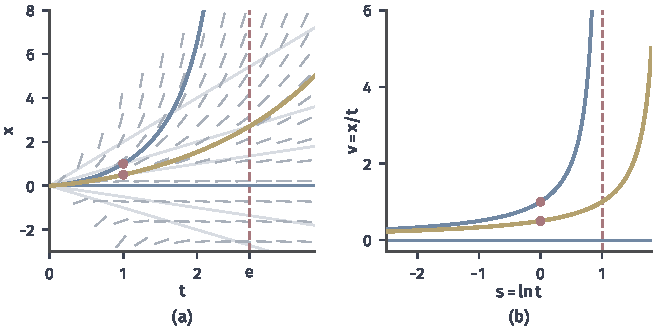
\includegraphics[width=112mm]{figures/06-differential-equations/01-ordinary-differential-equations/matplotlib/ivp-homogeneous-rays/figure.pdf}
 \caption{$\dot{x}=x/t+x^2/t^2$。(a)方向场在每条过原点的浅色射线上斜率相同。蓝线是$x(1)=1$的解$t/(1-\ln t)$，在$t=\mathrm{e}$（红色虚线）爆炸；黄线是$x(1)=0.5$的解$t/(2-\ln t)$；水平蓝线是$x\equiv 0$。(b)同样的解在坐标$s=\ln t$，$v=x/t$下满足自治方程$\mathrm{d}v/\mathrm{d}s=v^2$。}
 \label{fig:ivp-homogeneous-rays}
\end{BookInlineFigure}

图~\ref{fig:ivp-homogeneous-rays}(b)再做一次时钟变换$s=\ln t$，由式~\eqref{eq:ivp-homogeneous-reduced}得$\mathrm{d}v/\mathrm{d}s=v^2$。这正是第~\ref{sec:ivp-verification}节的爆炸方程，$v=1/(1-s)$。齐次型方程在缩放下的对称性，经过比值代换和对数时钟，变成了自治方程的时间平移不变性。

\paragraph{Bernoulli方程}
第二种代换把非线性项吸收掉。形如
\begin{equation}
 \dot{x}=p(t)\,x+q(t)\,x^{\alpha},\qquad\alpha\neq 0,\,1
 \label{eq:ivp-bernoulli}
\end{equation}
的方程称为\term{Bernoulli方程}（Bernoulli equation），$p$、$q$连续。$\alpha=0$或$1$时它本身就是线性的，所以排除这两种情况。

方程非线性，是因为$x^{\alpha}$与$x$次数不同。两边除以$x^{\alpha}$，得到$x^{-\alpha}\dot{x}=p\,x^{1-\alpha}+q$，左边恰好是$x^{1-\alpha}$导数的倍数。令
\begin{equation}
 w=x^{1-\alpha},
 \label{eq:ivp-bernoulli-substitution}
\end{equation}
则$\dot{w}=(1-\alpha)x^{-\alpha}\dot{x}$，代入得到线性方程
\begin{equation}
 \dot{w}=(1-\alpha)p(t)\,w+(1-\alpha)q(t).
 \label{eq:ivp-bernoulli-linear}
\end{equation}

\begin{lemma}[Bernoulli代换]
 \label{lem:ivp-bernoulli}
 在$x>0$的范围内，函数$x:I\to(0,\infty)$可微且解式~\eqref{eq:ivp-bernoulli}，当且仅当$w=x^{1-\alpha}:I\to(0,\infty)$可微且解式~\eqref{eq:ivp-bernoulli-linear}。
\end{lemma}

\begin{proof}
 因为$\alpha\neq 1$，$x\mapsto x^{1-\alpha}$是$(0,\infty)$到自身的连续可微双射，逆映射是$w\mapsto w^{1/(1-\alpha)}$，同样连续可微，所以两个方向都保持可微性。由链式法则，
 \[
 \dot{w}=(1-\alpha)x^{-\alpha}\dot{x}.
 \]
 把$\dot{x}$换成式~\eqref{eq:ivp-bernoulli}的右端，再用$x^{1-\alpha}=w$，就得到式~\eqref{eq:ivp-bernoulli-linear}。反方向把这一计算倒过来，用到$(1-\alpha)x^{-\alpha}\neq 0$。
\end{proof}

式~\eqref{eq:ivp-bernoulli-linear}系数依赖时间时，解法由第~\ref{chap:linear-differential-systems}章的积分因子给出。下面的例子系数为常数，可以用本节的方法完成。

Logistic方程$\dot{x}=x-x^2$是$p=1$，$q=-1$，$\alpha=2$的情形。代换$w=1/x$给出$\dot{w}=-w+1$。令$u=w-1$，$\dot{u}=-u$，所以$u=u_0\mathrm{e}^{-t}$，即
\[
 w(t)=1+(w_0-1)\mathrm{e}^{-t}.
\]
取$x_0=0.1$，$w_0=10$，$w=1+9\mathrm{e}^{-t}$，$x=1/w=\mathrm{e}^{t}/(\mathrm{e}^{t}+9)$，与式~\eqref{eq:ivp-logistic-solution}相同。图~\ref{fig:ivp-bernoulli-linearize}显示了这个代换的效果：$S$形的曲线变成了指数曲线。

\begin{BookInlineFigure}
 \centering
 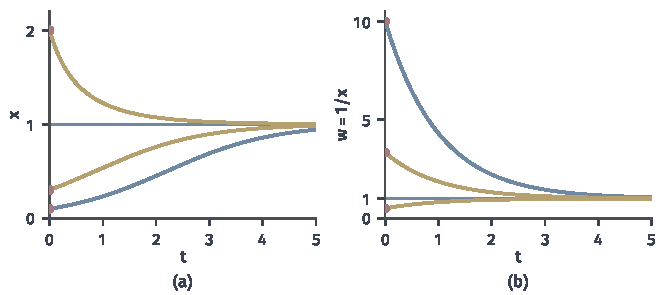
\includegraphics[width=112mm]{figures/06-differential-equations/01-ordinary-differential-equations/matplotlib/ivp-bernoulli-linearize/figure.pdf}
 \caption{代换$w=1/x$把Logistic方程变成线性方程。(a)$x_0=0.1$（蓝）与$x_0=0.3,\,2$（黄）的解。(b)同样三条解的$w=1/x=1+(w_0-1)\mathrm{e}^{-t}$，水平蓝线是$x\equiv 1$对应的$w\equiv 1$。平衡解$x\equiv 0$对应$w=\infty$，在(b)中没有位置。}
 \label{fig:ivp-bernoulli-linearize}
\end{BookInlineFigure}

这里的代换$w=1/x$对$x\neq 0$都可逆，所以负初值也能处理。$x_0=-0.5$时$w_0=-2$，$w=1-3\mathrm{e}^{-t}$，$w$在$t=\ln 3$处穿过零，对应$x\to-\infty$。原方程里的爆炸在$w$方程里只是平淡地穿过$0$，所以$w$的解可以继续，$x$的解却到此为止，这就是要核对取值范围的原因。而$x\equiv 0$对应$w=\infty$，代换把它排除在外，需要单独列出。

下一个例子演示符号的丢失。对$\dot{x}=x-x^3$，$\alpha=3$，代换$w=x^{-2}$给出$\dot{w}=-2w+2$，解是
\[
 w(t)=1+(w_0-1)\mathrm{e}^{-2t}.
\]
取$x_0=0.4$，$w_0=6.25$，$w=1+5.25\mathrm{e}^{-2t}$。若$x_0=-0.4$，$w_0$仍是$6.25$，得到完全相同的$w$。这时$w$只记录了$x$的大小，符号要从初值恢复：
\[
 x(t)=\operatorname{sign}(x_0)\,\bigl(1+5.25\mathrm{e}^{-2t}\bigr)^{-1/2}.
\]
由于$x\mapsto x^{-2}$在$\mathbb{R}\setminus\{0\}$上不是单射，代换只在$x>0$与$x<0$上分别可逆。解不能穿过$x=0$，否则$w$要经过无穷大。图~\ref{fig:ivp-bernoulli-sign}展示了这一点。

\begin{BookInlineFigure}
 \centering
 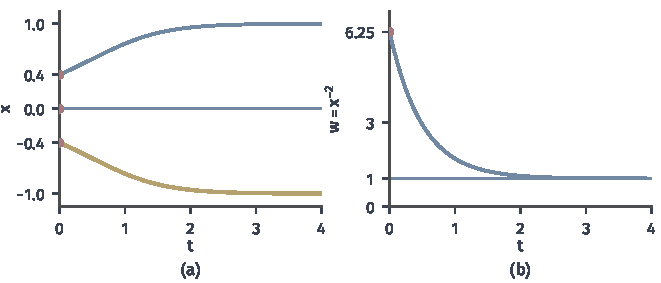
\includegraphics[width=112mm]{figures/06-differential-equations/01-ordinary-differential-equations/matplotlib/ivp-bernoulli-sign/figure.pdf}
 \caption{$\dot{x}=x-x^3$的代换$w=x^{-2}$。(a)初值$x_0=0.4$（蓝）与$x_0=-0.4$（黄）的解，以及平衡解$x\equiv 0$（红点是三个初值）。(b)$\pm 0.4$的解映成同一条$w=1+5.25\mathrm{e}^{-2t}$，水平蓝线对应$x\equiv\pm 1$。$x\equiv 0$在$w$中没有对应。}
 \label{fig:ivp-bernoulli-sign}
\end{BookInlineFigure}

最后看$\alpha<1$的情况，比如$\dot{x}=2\sqrt{x}$，$\alpha=1/2$，$p=0$，$q=2$。代换$w=\sqrt{x}$给出$\dot{w}=1$，线性方程的解唯一，$w=w_0+t$。可是上一小节已经看到，$x_0=0$时原方程有无穷多解。矛盾来自引理~\ref{lem:ivp-bernoulli}的范围：$x\mapsto\sqrt{x}$在$x=0$处不可微，等式$\dot{w}=\dot{x}/(2\sqrt{x})$在那里没有意义，解一旦碰到$x=0$，新旧方程就不再等价。形式上的化简可以很干净，它给出的却不一定是原问题的全部解。

下表整理这些代换的适用范围。
\begin{BookInlineTable}
 \centering
 \caption{变量代换的核验项}
 \label{tab:ivp-substitution}
 \begin{tabular}{llll}
 \toprule
 方程 & 代换 & 可逆范围 & 需单独检查 \\
 \midrule
 $\dot{x}=F(x/t)$ & $v=x/t$ & $t\neq 0$ & 直线解$x=v^{\star}t$ \\
 $\dot{x}=x-x^2$ & $w=1/x$ & $x\neq 0$ & $x\equiv 0$，$w$过零 \\
 $\dot{x}=x-x^3$ & $w=x^{-2}$ & $x>0$或$x<0$ & $x\equiv 0$，符号 \\
 $\dot{x}=2\sqrt{x}$ & $w=\sqrt{x}$ & $x>0$ & 碰到$x=0$的解 \\
 \bottomrule
 \end{tabular}
\end{BookInlineTable}
